\documentclass{article}

\usepackage{fancyhdr}
\usepackage{extramarks}
\usepackage{amsmath}
\usepackage{amsthm}
\usepackage{amsfonts}
\usepackage{tikz}
\usepackage{algpseudocode}
\usepackage{titlesec}
\usepackage[T1]{fontenc}  % let \textsc in \subsection work well.
\usepackage{graphicx}
\usepackage{hyperref}
\usepackage[Algorithmus]{algorithm}
\usepackage{algorithmicx} % use this. this is pretty.
\usepackage{subcaption}
\usepackage{float}
\usepackage{booktabs}
\usepackage{textcomp}

\usetikzlibrary{automata,positioning}

%
% Basic Document Settings
%

\topmargin=-0.45in
\evensidemargin=0in
\oddsidemargin=0in
\textwidth=6.5in
\textheight=9.0in
\headsep=0.25in

\linespread{1.1}

\pagestyle{fancy}
\chead{\hmwkTitle}
\rhead{\firstxmark}
\lfoot{\lastxmark}
\cfoot{\thepage}

\renewcommand\headrulewidth{0.4pt}
\renewcommand\footrulewidth{0.4pt}

\setlength\parindent{0pt}

%
% Create Problem Sections
%

\newcommand{\enterProblemHeader}[1]{
    \nobreak\extramarks{}{Question \arabic{#1} continued on next page\ldots}\nobreak{}
    \nobreak\extramarks{Question \arabic{#1} (continued)}{Question \arabic{#1} continued on next page\ldots}\nobreak{}
}

\newcommand{\exitProblemHeader}[1]{
    \nobreak\extramarks{Question \arabic{#1} (continued)}{Question \arabic{#1} continued on next page\ldots}\nobreak{}
    \stepcounter{#1}
    \nobreak\extramarks{Question \arabic{#1}}{}\nobreak{}
}

\setcounter{secnumdepth}{0}
\newcounter{partCounter}
\newcounter{homeworkProblemCounter}
\setcounter{homeworkProblemCounter}{1}
\nobreak\extramarks{}{}\nobreak{}

%
% Homework Problem Environment
%
% This environment takes an optional argument. When given, it will adjust the
% problem counter. This is useful for when the problems given for your
% assignment aren't sequential. See the last 3 problems of this template for an
% example.
%
\newenvironment{homeworkProblem}[1][-1]{
    \ifnum#1>0
    \setcounter{homeworkProblemCounter}{#1}
    \fi
    \section{Question \arabic{homeworkProblemCounter}}
    \setcounter{partCounter}{1}
    \enterProblemHeader{homeworkProblemCounter}
    }{
    \exitProblemHeader{homeworkProblemCounter}
}

%
% Homework Details
%   - Title
%   - Due date
%   - Class
%   - Section/Time
%   - Instructor
%   - Author
%

\date{}
\newcommand{\hmwkTitle}{Lightweight Transformers for Text Generation}
\newcommand{\hmwkClass}{Distillation, Pruning, and Quantization of BART-large and GPT-2}

%
% Title Page
%

\title{
    \vspace{2in}
    \textmd{\textbf{\huge \hmwkTitle}}\\
    \vspace{0.1in}
    \textmd{\textit{\fontsize{15}{30}\selectfont \hmwkClass}}\\
    \vspace{0.1in}
    \author{
        \textbf{Six Degrees of Inner Turbulence} \\\\
        {
            \begin{tabular}{c|c}
                \toprule
                \textbf{Name} & \textbf{UFID} \\
                \midrule
                GuangYan An & 9853-4118 \\
                Xiaolin Zheng & 5400-7588 \\
                \bottomrule
            \end{tabular}
        }
    }
    \vspace{3in}
}


\renewcommand{\part}[1]{\textbf{\large Part \Alph{partCounter}}\stepcounter{partCounter}\\}

%
% Various Helper Commands
%

% Useful for algorithms
\newcommand{\alg}[1]{\textsc{\bfseries \footnotesize #1}}

% For derivatives
\newcommand{\deriv}[1]{\frac{\mathrm{d}}{\mathrm{d}x} (#1)}

% For partial derivatives
\newcommand{\pderiv}[2]{\frac{\partial}{\partial #1} (#2)}

% Integral dx
\newcommand{\dx}{\mathrm{d}x}

% Alias for the Solution section header
\newcommand{\solution}{\textbf{\large Solution}}

% Probability commands: Expectation, Variance, Covariance, Bias
\newcommand{\E}{\mathrm{E}}
\newcommand{\Var}{\mathrm{Var}}
\newcommand{\Cov}{\mathrm{Cov}}
\newcommand{\Bias}{\mathrm{Bias}}

% Note: Section number
\setcounter{secnumdepth}{3}

\begin{document}

    \maketitle
    \pagebreak

    \tableofcontents
    \pagebreak

    \section{Introduction}
    \hspace*{1em} Text generation systems play a critical role in improving user efficiency in applications like typing assistants, chatbots, and new digests. Traditional methods, often based on n-gram or rule-based models, struggle with understanding complex sentences and providing accurate suggestions over longer contexts. The emergence of transformer-based models has transformed Natural Language Processing (NLP). Models like BERT, BART, and GPT-2 leverage bidirectional context, enabling more accurate predictions. Transformers also benefit from large pre-trained models and extensive datasets, but they come with the drawback of requiring significant computational resources, which can limit their use in real-time applications.

    \hspace*{1em} Many companies, such as Microsoft, Meta, and Apple, have developed their own text completion / summarization systems. However, these solutions often have limitations, such as device or platform restrictions. Our motivation is to create a context-aware text completion / summarization system that balances quality, speed, and efficiency, working across platforms without sacrificing performance.

    \hspace*{1em} Regarding these challenges, we employed several established techniques to reduce the size of pre-trained models and enhance model inference speed, while keeping accuracy loss within acceptable limits. These techniques include knowledge distillation, movement pruning, and quantizations. In the following sections, we will present the development, internals, and outcomes of the optimized pre-trained models. Section 2 discusses the related work. Section 3 presents knowledge distillation, movement pruning, and quantization (including post-training quantization, PTQ and quantization-aware training, QAT) methodology. Section 4 shares the knowledge distiller, movement pruning techniques, and quantization implementations. It also summarizes the final and overall performance, inference time, and memory footprint generated and evaluated by using our distillation-pruning-quantization pipelines on pre-trained Transformer models. Section 5 concludes this project and discusses various potential future improvement we have observed and summarized in these months during the project.

    \section{Related Work}
    \subsection{Knowledge Distillation}
    \hspace*{1em} Hinton et al. proposed the concept of knowledge distillation\cite{Hinton2015}, providing the basis for model compression and optimization. Knowledge distillation uses soft targets of the teacher model as the learning target for the smaller student model by minimizing the KL divergence between the output probability distributions of the teacher and the student. After that, FitNets\cite{romero2015fitnets} proposed using intermediate representations, such as feature maps and hidden states, of the teacher model as a guidance for students to learn internal representations. Students not only imitate the final outputs of the teachers, but also replicate their details. Then, \texttt{DistilBERT}\cite{sanh2019distilbert} applied this technique to \texttt{BERT}, a Transformer model, reducing its parameters by 40\% percent while retaining more than 97\% of the performance on various workloads. Subsequently, Shleifer and Rush extended knowledge distillation techniques to the field of text summarizations\cite{shleifer2020distillation}. Their approach introduced task-related techniques to distill large summarization models, such as \texttt{T5} and \texttt{BART}, into smaller models, with a smaller model inference time. These researches demonstrate that by effectively extracting and transferring knowledge from different layers of the teacher model, knowledge distillation can significantly reduce model footprint and inference time, making models adaptable to various application scenarios.

    \subsection{Pruning}
    \hspace*{1em} Early pruning strategy focused on sparsifying weight matrices by removing weights with small values, which is unstructured pruning\cite{han2015learning}. For Transformers, structured pruning is applied to optimize the self-attention and feed-forward neural network components. This approach calculates importance scores to select necessary attention heads and drop the others\cite{michel2019sixteen} without significantly degrading the model performance. After that, movement pruning\cite{sanh2020movement} was proposed to dynamically adjust the pruning strategy during training or fine-tuning process according to gradient information, improving the overall model precision and robustness after pruning. This strategy can be applied to both unstructured and structured pruning, which is flexible. Famous real-world model pruning implementations include \texttt{torch.nn.utils.prune}, which contains both unstructured and structured pruning. For unstructured pruning, the implementation leverages random masks or weight thresholds to drop weights in a parameter-by-parameter manner. Structured pruning is a larger-granularity pruning that removes neurons, convolution kernels, or attention heads.

    \subsection{Quantization}
    \hspace*{1em} Quantization includes weight quantization and activation quantization. In recent years, 8-bit weight and activation quantization has become mainstream in Transformer models, since quantizing a 32-bit float point Transformer to an 8-bit model can largely reduce the model footprint and inference cost while retaining high precision. For instance, \texttt{Q8BERT}\cite{zafrir2019q8bert} proposed a quantized 8-bit \texttt{BERT} model, reducing the model size by approximately 4x by applying quantization-aware training. Furthermore, \texttt{TernaryBERT}\cite{zhang2020ternarybert} uses a ternary quantization mechanism, and the weights of the model only take values in \texttt{\{-1, 0, 1\}}, further achieving a higher compression rate while retaining the performance. Real-world implementations of quantization include \texttt{TorchQuantization}, which provides implementations of post-training quantization and quantization-aware training. Post-training quantization requires the offline collection of calibration data to generate precise scale factors after converting the model. For quantization-aware training, \texttt{TorchQuantization} supports inserting fake quantization modules in the model and significantly improves the performance of low-precision models by simulating and propagating quantized model loss to optimize the weights of the quantized model.

    \section{Methodology}
    \subsection{Experimental Setup}
    \hspace*{1em} We used a subset of OpenWebText dataset\cite{OpenWebText2019}, an open-source replication of OpenAI's WebText, for autoregressive text prediction and a BBC news dataset containing original posts and their corresponding summarizations for text summarization. We utilized HuggingFace's \texttt{transformers}\cite{wolf-etal-2020-transformers} library, which provides the pre-trained definitions for BART and GPT-2 models, as well as the \texttt{Trainer} and \texttt{Seq2SeqTrainer} APIs, to fine-tune these models during training. The latter allowed us to focus more on optimizing the models rather than implementing training routines (trainer, checkpointing, etc.) from scratch. The model optimization pipelines were trained and evaluated on an A100 GPU with 40GB memory on Google Colab and required approximately 5 hours of runtime since only a small subset of the original dataset was used (We could only afford this setting). Before applying the optimizations, we first fine-tuned the pre-trained models on the prepared datasets to warm them up, also for later performance comparison.

    \subsection{Knowledge Distillation}
    \hspace*{1em} Knowledge Distillation was proposed in 2015 as a technique for transferring knowledge from a large, complex model (teacher model) to a smaller, more efficient model (student model). The key idea is that the student model can achieve comparable performance to the teacher model by learning soft labels of the teacher: probability distributions instead of learning the true labels only. This allows the student to learn intermediate representations from the teacher. The loss function of knowledge distillation can be expressed as:

    \begin{equation}
        L_{\text{KD}} = \alpha L_{\text{CE}}(y, \hat{y}) + (1 - \alpha) T^2 L_{\text{KL}}(q_t, q_s)
    \end{equation}

    \hspace*{1em} In the above expression, $L_{\text{CE}}(y, \hat{y})$ represents the loss between prediction probability distribution $\hat{y}$ and true labels $y$ using traditional cross entropy loss. $L_{\text{KL}}(q_t, q_s)$ expresses the difference between the output distributions of the student and the teacher. $T$ is the temperature hyperparameter, used to soften softmax distributions of $q_t$ and $q_s$. Finally, $\alpha$ controls the balance between different kinds of losses.

    \hspace*{1em} BART-large-CNN\cite{lewis2020BART} was pre-trained and fine-tuned on the CNN Daily Mail dataset and has a powerful ability of text summarization. It has 12 Transformer encoder layers and 12 Transformer decoder layers, the model being in total of 1.51GB. GPT-2\cite{radford2019language} was a pre-trained autoregressive decoder model using a causal language masking objective, containing 12 Transformer decoder layers with a total size of 0.548 GB. We extracted the layers 0, 2, 5, 7, 9, 11 from the encoder / decoder to form the student's encoder / decoder, thereby halving the model's storage. Weight state dicts of these layers are also loaded to avoid pre-training from scratch.

    \hspace*{1em} In our implementation, we chose to use \texttt{MSE} to match the logits output at each hidden layer as described in Chen et al. (2020)\cite{shleifer2020distillation} since this can encourage the student to even match teacher hidden states. The loss function is updated as follows, where we want the student to generate hidden layers weights as comparable to the teacher as possible:

    \begin{equation}
        L_{\text{KD}} = \alpha L_{\text{CE}}(y, \hat{y}) + \beta L_{\text{MSE}(hid_t, hid_s)} + \gamma T^2 L_{\text{KL}}(q_t, q_s)
    \end{equation}

    \hspace*{1em} For the $\alpha, \beta, \gamma, T$ hyperparameters, we set $\alpha$ to 0.1, $\beta$ to 3, $\gamma$ to 0.8, and $T$ to 2, since we aim to maximize the hidden state learning by the student from the teacher.

    \begin{figure}[hbpt]
        \centering
        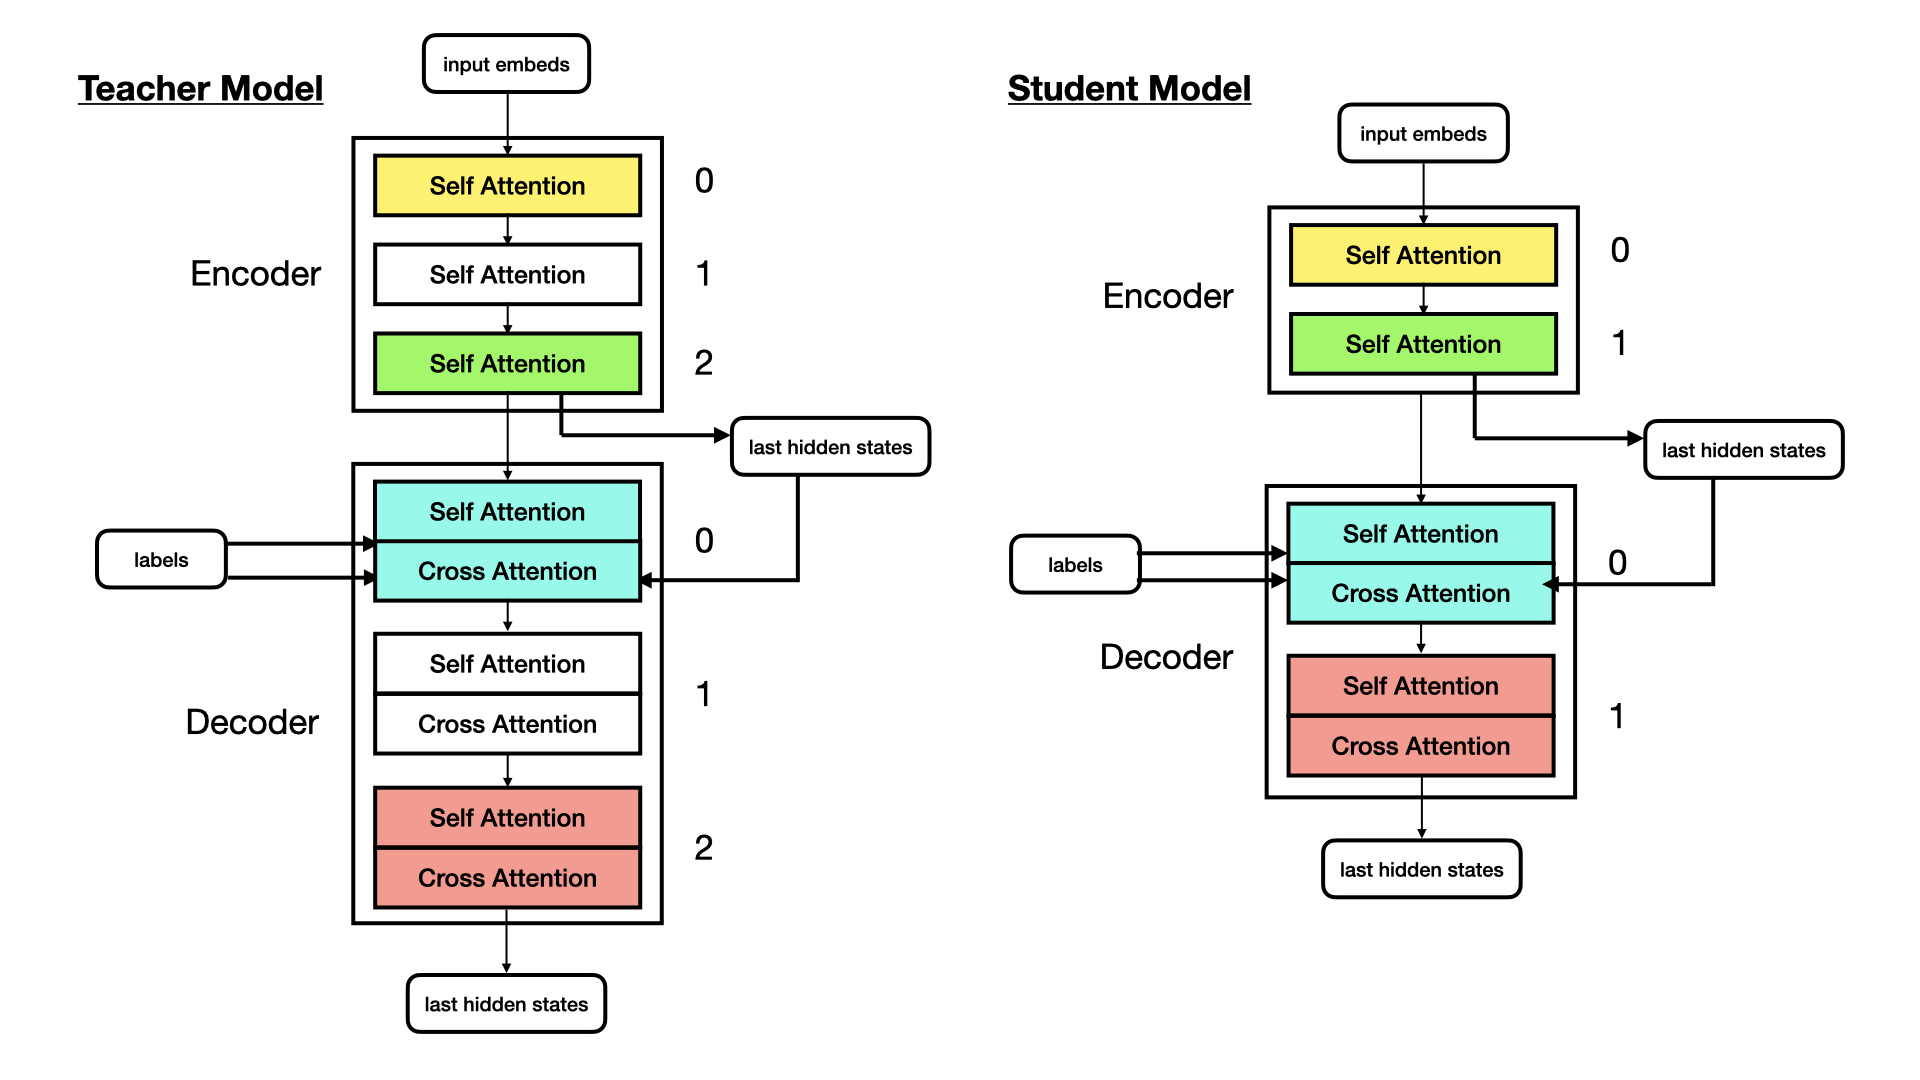
\includegraphics[width=1\textwidth]{pics/pa/0.001}
        \caption{Example of distillation of Encoder-Decoder model, e.g. BART-large}
        \label{fig:sub1}
    \end{figure}

    \begin{figure}[hbpt]
        \centering
        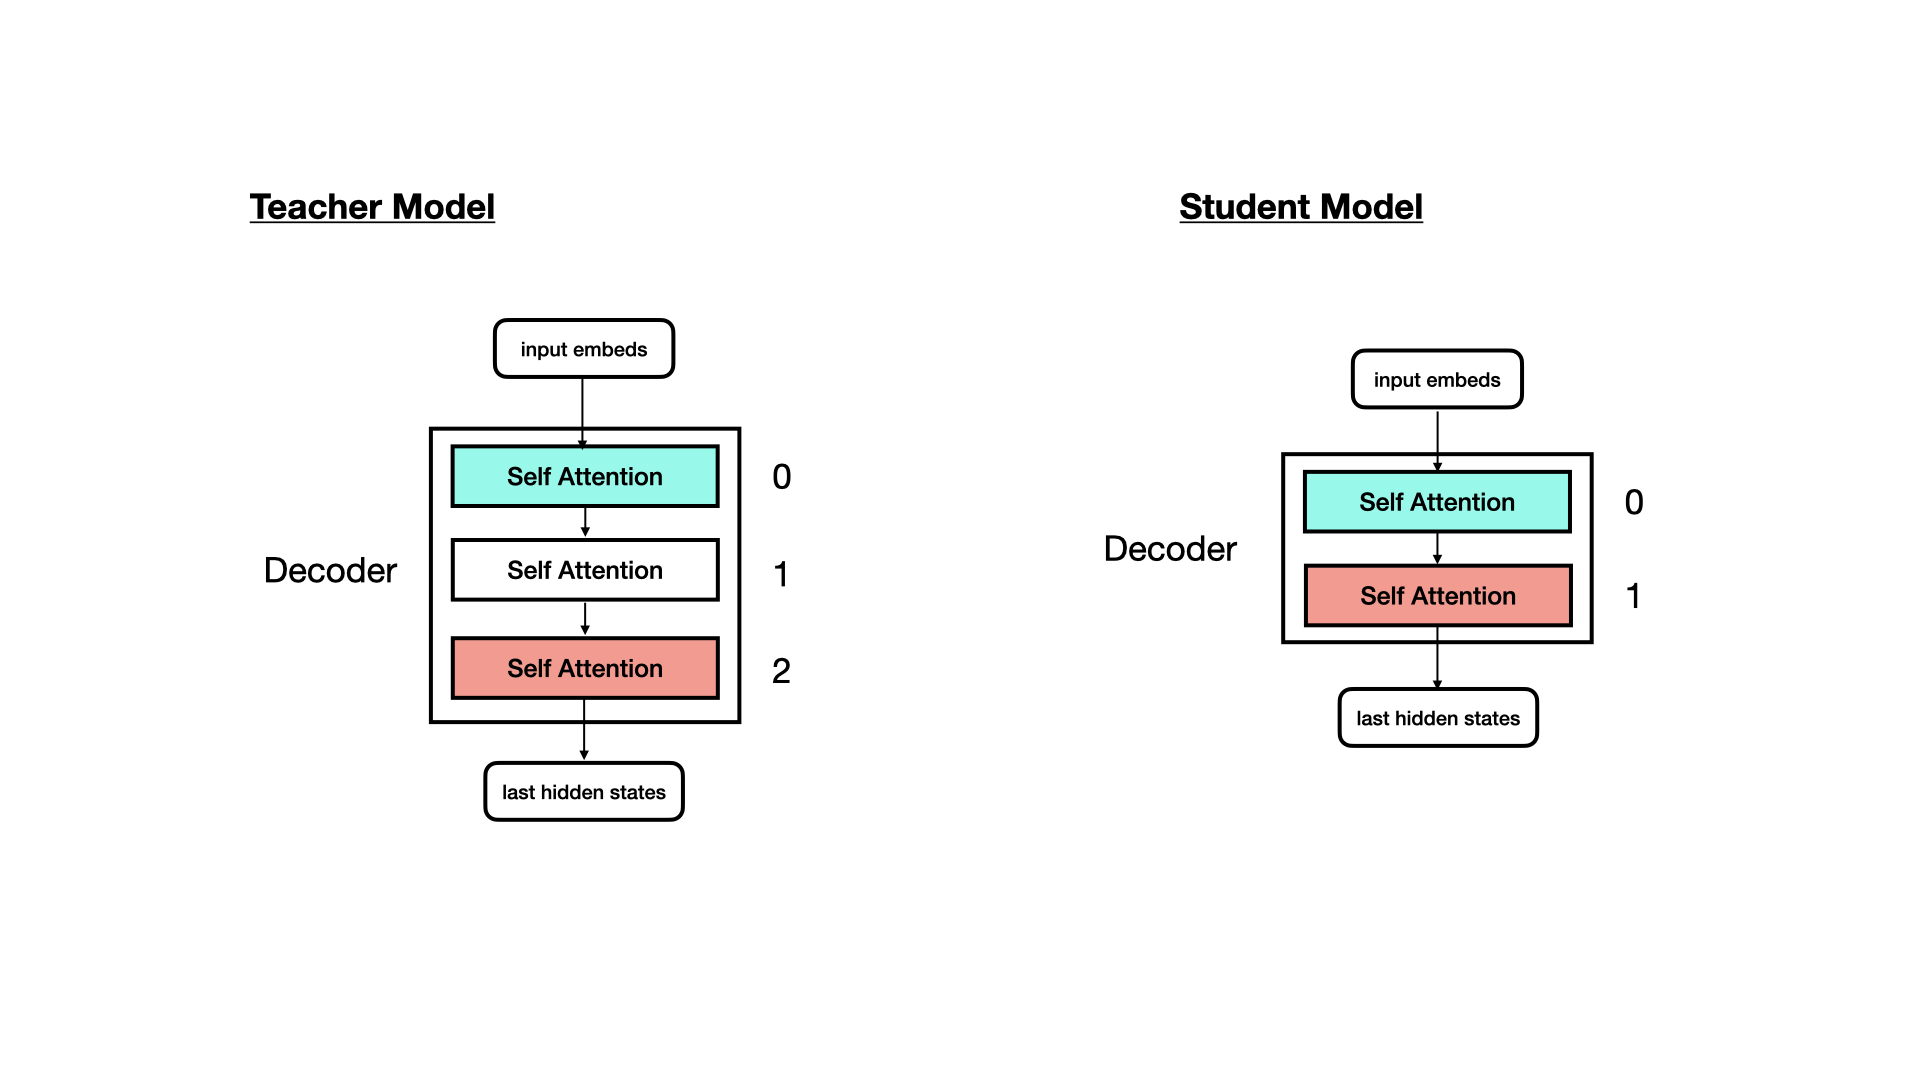
\includegraphics[width=1\textwidth]{pics/pa/0.002}
        \caption{Example of distillation of Decoder-Only model, e.g. GPT-2}
        \label{fig:sub2}
    \end{figure}

    \hspace*{1em} As shown in Figure~\ref{fig:sub1}, this image illustrates an example encoder-decoder Transformer (e.g. BART) teacher model with 3 layers for each on the left. On the right a distilled student model extracts the first and last layers of the teacher's encoder and decoder (using the same colors) and forms a new encoder and decoder. Arrows in this figure show the data flow: \texttt{input embeds} are the text embedding input, which will become \texttt{Q,K,V} in encoders. Encoder's last hidden layer states will be transformed to \texttt{K,V} used in cross-attention of decoder layers, and the \texttt{labels} are fed as \texttt{Q,K,V} in self-attention but as \texttt{Q} only in cross-attention of decoder layers.

    \hspace*{1em} Figure~\ref{fig:sub2} presents an example 3-layer decoder-only Transformer (e.g. GPT-2) teacher model on the left, which is much simpler than the previous one since decoder-only models can choose not to use cross-attention, meaning it only leverages self-attention. On the right a distilled student model extracts the first and last layers of the teacher's decoder (using same colors) and forms a new decoder. \texttt{input embeds} will become \texttt{Q,K,V} in decoders. Finally the final logits generated by the decoder will be compared with the original text embeddings using cross entropy to calculate the loss because of autoregression.


    \subsection{Movement Pruning}
    \hspace*{1em} Pruning is a model optimization technique aimed at reducing the size and computational complexity of deep learning models by removing less important parameters or structures. There are several different classification approaches for pruning, including by granularity (weight, neuron, channel, layer), by timing (pre-training, during training, post-training), and by target (structural, unstructural). Our pruning strategy focuses on neurons in FFN layers and attention heads in \texttt{QKV} projection layers. Specifically, we train pruning masks for both FFN and \texttt{QKV} projections separately, and finally perform pruning using the masks. Therefore, our approach can be categorized as structural movement pruning, taking neurons and attention heads as the minimum granularity.

    \hspace*{1em} We assign a uniformly drawn score to each neuron in an FFN layer and to each head in an attention layer. Each time during forward passes, we use a threshold \texttt{K} to select the top \texttt{K} smallest scores and drop the corresponding neurons and attention heads by transforming the scores into masks. Regarding neurons and attention heads as pruning granularity, we should notice that once we have determined which attention head is useless, we should remove that same head from all \texttt{QKV} projections and the final output projection in the current attention. Also for FFN layers that contain two linear layers \texttt{fc1} and \texttt{fc2}, once we have decided which neuron can be pruned in \texttt{fc1}, we must remove the corresponding neuron defined in \texttt{fc2}.  Therefore, we call our trained scores ``shared score'' or ``shared mask'', since they are shared among \texttt{QKV} attention projections, and among FFN layers.

    \hspace*{1em} During the training process in order to find the best shared masks in the Transformer, we will apply the current shared masks in forward and backward passes to train learnable shared masks. However, the masking operation is not differentiable since it zeros out all corresponding attention heads and set them to zero as inactive heads during forward passes. To solve this, we applied STE, which stands for straight-through estimator techniques to estimate gradients during backward passes so that the scores can be updated properly. Therefore, the most important neuron or attention heads must have the highest score theoretically due to natural selection. Additionally, we implemented a dynamic threshold scheduler for the movement pruning trainer. For instance, in our setup, we aim to prune 30\% of the attention heads in the Transformer and 60\% of the neurons in FFN layers. To minimize abrupt performance degradation, the scheduler gradually increases the total masking threshold from 0\% to 30\% following a cubic curve for masked attention heads. The thresholds will reach their peek at 85\% of the training progress and stay at the peek until the end and use the remaining 15\% of the progress for fine-tuning, as shown in Figure~\ref{fig:sub3}.

    \begin{equation}
        \text{threshold} = \text{threshold}_{\text{final}} - \left( \text{threshold}_{\text{final}} - \text{threshold}_{\text{init}} \right) \cdot (1 - progress)^3
    \end{equation}

    \hspace*{1em} Figure~\ref{fig:two_images_subcaption} shows a sample pruning result for an FFN layer on the left, alongside the results for pruning self-attention and cross-attention in a decoder layer. Darker colors indicate that the corresponding neuron or attention head has been pruned.

    \begin{figure}[hbpt]
        \centering
        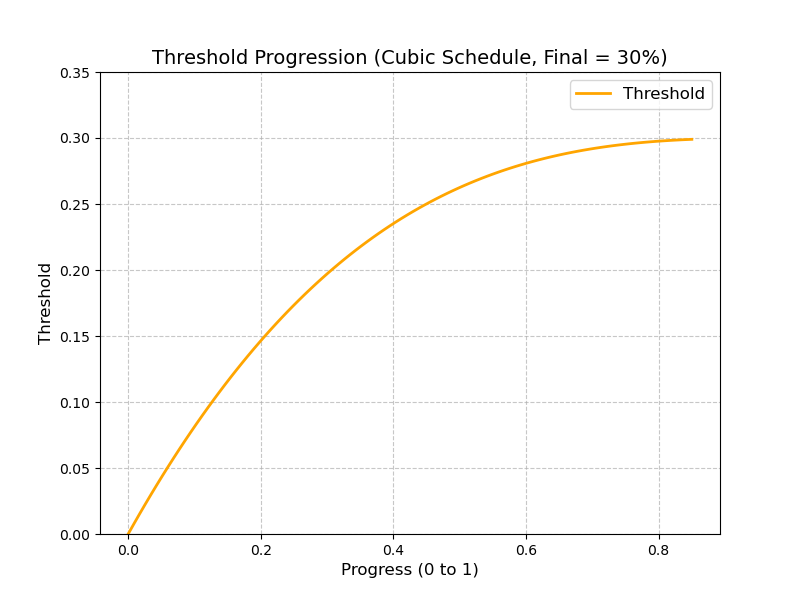
\includegraphics[width=0.6\textwidth]{pics/pa/1}
        \caption{Movement Threshold Scheduler for Attention Layers}
        \label{fig:sub3}
    \end{figure}

    \begin{figure}[h!]
        \centering
        \begin{subfigure}[b]{0.55\textwidth}
            \centering
            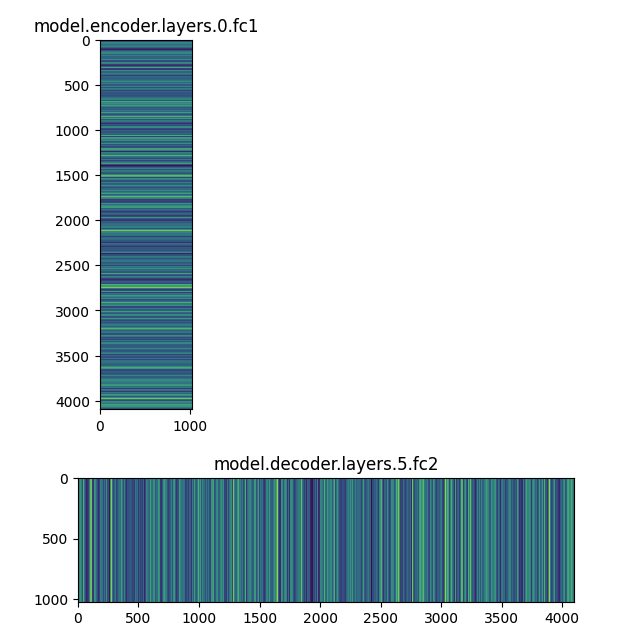
\includegraphics[width=\textwidth]{pics/pa/pruning1}
            \caption{Sample Neuron Pruning}
            \label{fig:subfig1}
        \end{subfigure}
        \hspace{0.02\textwidth}
        \begin{subfigure}[b]{0.35\textwidth}
            \centering
            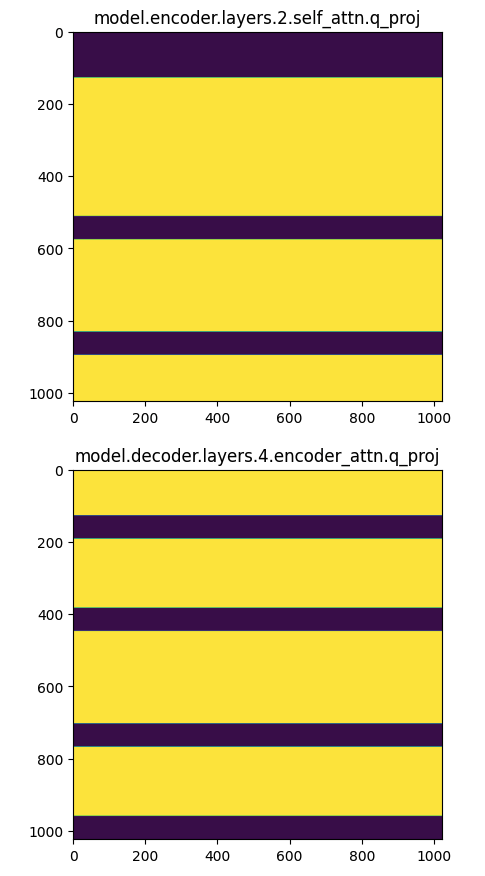
\includegraphics[width=\textwidth]{pics/pa/pruning2}
            \caption{Sample Attention Head Pruning}
            \label{fig:subfig2}
        \end{subfigure}
        \caption{Samples: Movement Pruning Distribution}
        \label{fig:two_images_subcaption}
    \end{figure}

    \subsection{Quantization}
    \hspace*{1em} Quantization can reduce the precision of numbers used to present parameters or activations. By converting high-precision floating-point numbers (FP32, FP64) to lower precision (INT8, FP16), quantization reduces the memory footprint and computational requirements of a model, making it more efficient for deployment on resource-constrained devices like edge or mobile devices. Types of quantization include PTQ, standing for post-training quantization, and QAT, short for quantization-aware training. To map FP32, for instance, to INT8, we can convert floating point values into quantized space using linear mapping strategy, as expressed below:


    \begin{align}
        r &= S(q-Z) \\
        q &= \operatorname{round}\left(\frac{r}{S} + Z\right)
    \end{align}

    , where $r$ and $q$ are the number before and after quantization; $S$ and $Z$ are scale and zero-point. The linear mapping is referred to as symmetric or asymmetric mapping, depending on whether $Z$ is zero, as shown in Figure~\ref{fig:sub4}, where a symmetric range is converted to a symmetric INT8 range on the left and an asymmetric range is mapped to an asymmetric INT8 range.

    \begin{figure}[hbpt]
        \centering
        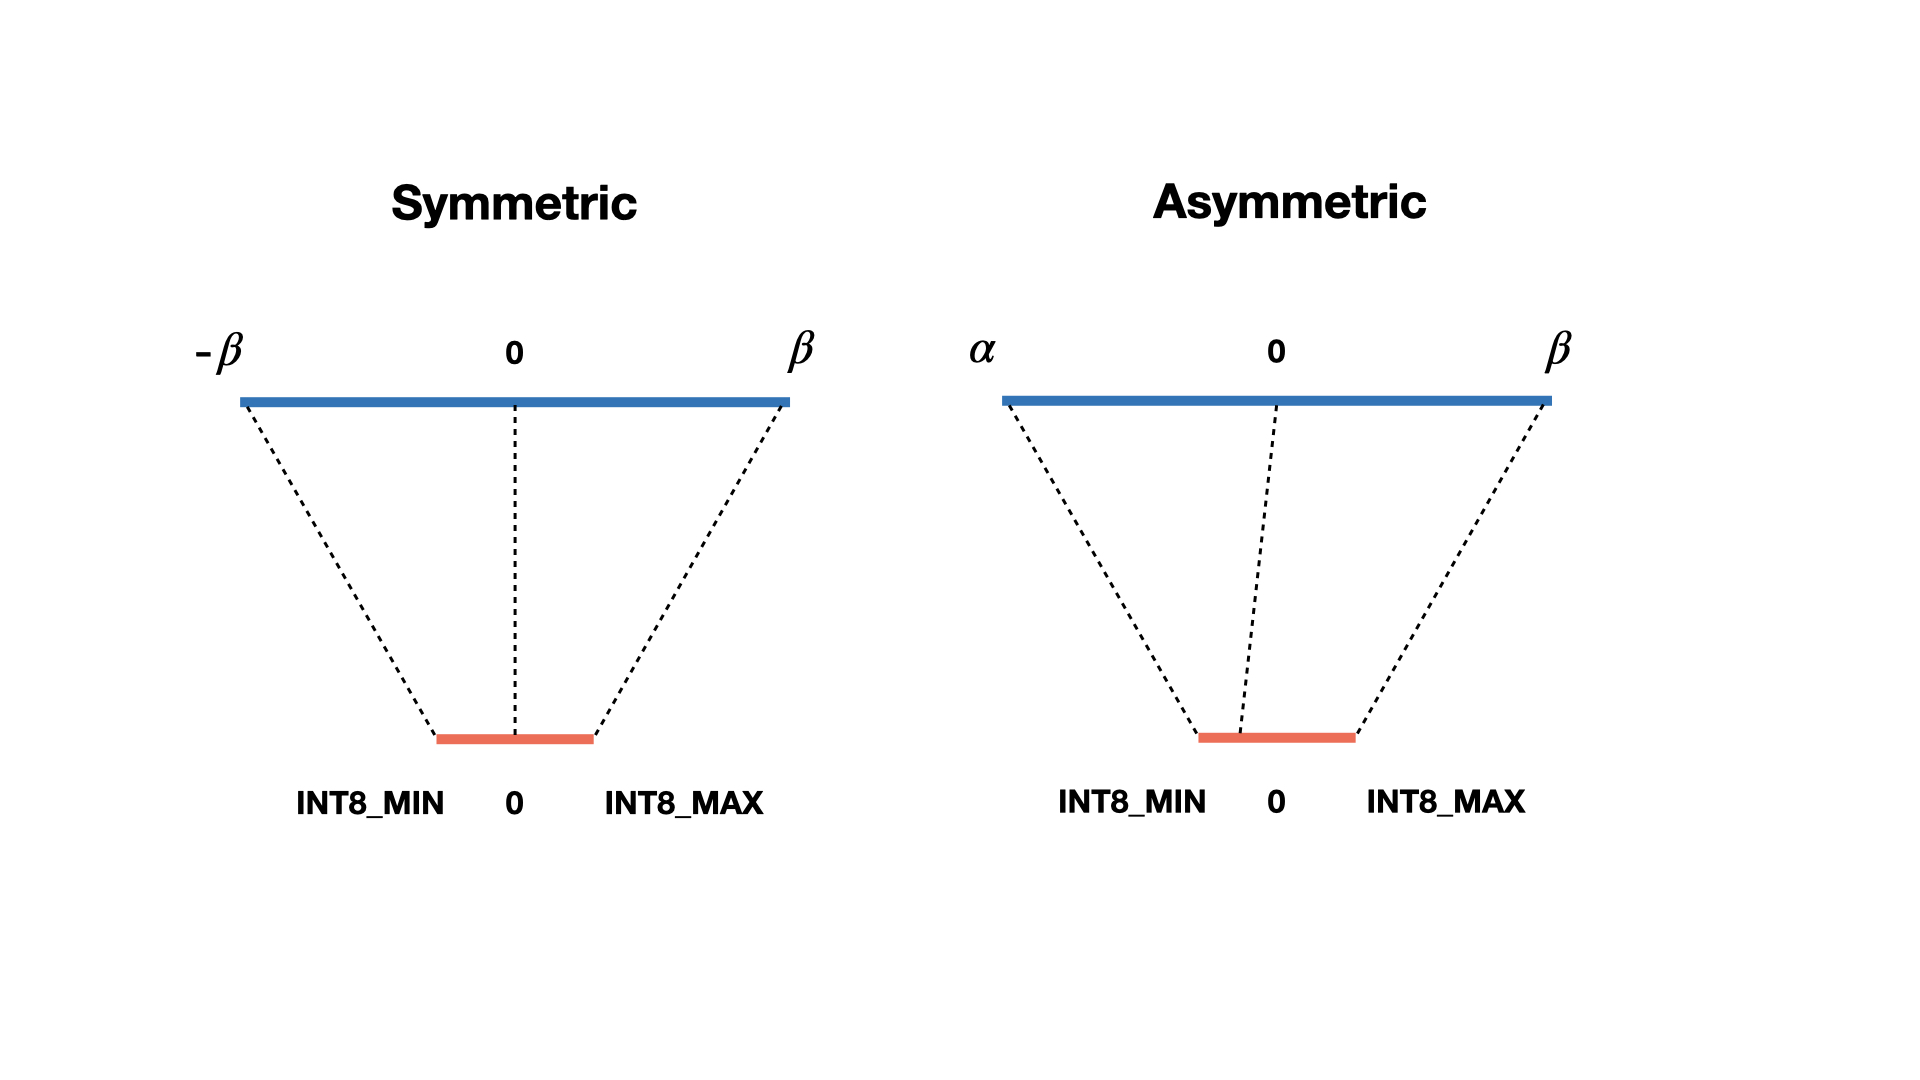
\includegraphics[width=1\textwidth]{pics/pa/0.003}
        \caption{Linear Mapping with or without Zero-point}
        \label{fig:sub4}
    \end{figure}

    \hspace*{1em} After mapping FP32 to INT8, which is PTQ, the memory footprint is significantly reduced; however, this comes at the cost of precision and performance degradation. To compensate for the degradation, calibration can be performed by feeding real data into the quantized model to estimate and adjust weight ranges.

    \hspace*{1em} Another approach for the model to adjust for quantization errors is to use online quantization techniques, for instance, QAT, instead of the offline PTQ method. QAT involves training the model with quantization simulated during the process to improve performance after quantization. Despite weights being quantized to INT8, during the forward process weights are still represented as FP32 to adjust for quantization errors. After quantization-aware training, the model learns to compensate for quantization errors, ensuring minimal performance degradation, followed by PTQ after training to convert the model to an INT8 format, and inference is performed using INT8 precision.

    \hspace*{1em} Our approach follows the above description, performing QAT first, followed by PTQ. To implement QAT, We designed a \texttt{QLinear} layer to substitute the original \texttt{torch.nn.Linear} layers to perform quantization-aware training. There was a similar problem as described in the pruning section: the linear mapping process, as we call it \texttt{affine}, leveraging \texttt{round} and \texttt{clamp} operations, is non-differentiable. We applied the same approach described above: STE to estimate the backward gradient for our \texttt{QLinear} layers to learn and gradually adjust for quantization errors. We rewrote the backward function for the $XW + b$ linear operation, plugging in \texttt{affine} and \texttt{deaffine} logic for $W$ parameters during forward and backward passes. Another operation worth mentioning is that we did not assign zero-points in \texttt{affine} and \texttt{deaffine} since during experiments we found the performance of the models was better using symmetric quantization perhaps due to weight distribution in the pre-trained models.


    \section{Experimental Results}
    \subsection{Knowledge Distillation}
    \hspace*{1em} We have evaluated the performance, inference time, and the reduction of storage for our distiller with the settings discussed above. As the table~\ref{tab:BART_comparison} shows below, the distiller for BART-large-CNN on text summarization had a good result: not only did our student have nearly the same rouge scores as the teachers', but it also had 26.7\% inference time reduction and 43\% model size reduction. The rouge scores range from 0 to 1, with higher values indicating better quality. Please note that the model size reduction is less than 50\% but that is normal since Transformer models have a shared embedding layer above the encoder to transform text ids to text embeddings,  % (bs, seq_len) -> (bs, seq_len, n_dim)
    and another linear language modeling head layer below the decoder to map hidden states to vocabulary logits. % (bs, seq_len, n_dim) -> (bs, seq_len, vocab_sz)

    \begin{table}[h!]
        \centering
        \begin{tabular}{lcc}
            \toprule
            \textbf{Name}         & \multicolumn{2}{c}{\textbf{BART-large-CNN}} \\ \midrule
            \textbf{Metric}       & \textbf{Teacher Model} & \textbf{Student Model} \\ \midrule
            Encoder Layers        & 12                     & 6                     \\
            Decoder Layers        & 12                     & 6                     \\
            ROUGE-1 Score         & 0.717                  & 0.716                  \\
            ROUGE-2 Score         & 0.617                  & 0.617                  \\
            ROUGE-L Score         & 0.541                  & 0.551                  \\
            ROUGE-Lsum Score      & 0.559                  & 0.604                  \\
            Inference Time        & 59.25s                 & 43.43s                 \\
            Model Size            & 1.51GB                 & 0.86GB                 \\ \bottomrule
        \end{tabular}
        \caption{Comparison of Teacher and Student Models for BART-large-CNN}
        \label{tab:BART_comparison}
    \end{table}

    \hspace*{1em} The result of distiller for GPT-2 are shown below in the table~\ref{tab:gpt2_comparison}. Since we use GPT-2 for text prediction and it is an autoregressive decoder-only model, perplexity was used to evaluate model performance. The lower the perplexity score, the better the model's predicted probability distribution matches the true data distribution, indicating higher quality in generated text under certain conditions. The table suggests that the perplexity score downgraded from 18.25 to a ``more perplexing'' 31.98, which we believe it is due to the small size of the dataset, and because on text generation we did not train it to full convergence due to a lack of resources. However, the inference time shows 19\% reduction, with the model reduced by 43\% (the latter one is same as the result from BART-large-CNN).

    \begin{table}[h!]
        \centering
        \begin{tabular}{lcc}
            \toprule
            \textbf{Name}         & \multicolumn{2}{c}{\textbf{GPT-2}} \\ \midrule
            \textbf{Metric}       & \textbf{Teacher Model} & \textbf{Student Model} \\ \midrule
            Decoder Layers        & 12                     & 6                     \\
            Perplexity            & 18.25                  & 31.98                  \\
            Inference Time        & 43.18s                 & 34.95s                 \\
            Model Size            & 0.548GB                & 0.31GB                 \\ \bottomrule
        \end{tabular}
        \caption{Comparison of Teacher and Student Models for GPT-2}
        \label{tab:gpt2_comparison}
    \end{table}

    \subsection{Movement Pruning}
    \hspace*{1em} We applied only our pruner on the fine-tuned BART-large-CNN model without applying distillation to show pruning results. The table~\ref{tab:BART_comparison_pruning} below shows 35\% of storage reduction and about 4\% of rouge score loss, which means our pruning strategy works. A reflection on the pruning strategy is that, we use learnable scores (masks), train those masks, and apply those masks during training to get the most valuable neurons / attention headers, which has similar semantics as QAT using quantization-aware weights during training. Besides, the STE strategy is applied as well both in pruning and in QAT.

    \begin{table}[h!]
        \centering
        \begin{tabular}{lcc}
            \toprule
            \textbf{Name}         & \multicolumn{2}{c}{\textbf{BART-large-CNN}} \\ \midrule
            \textbf{Metric}       & \textbf{Original} & \textbf{Pruned} \\ \midrule
            Encoder Layers        & 12                     & 12                     \\
            Decoder Layers        & 12                     & 12                     \\
            ROUGE-1 Score         & 0.717                  & 0.713                  \\
            ROUGE-2 Score         & 0.617                  & 0.612                  \\
            ROUGE-L Score         & 0.541                  & 0.530                  \\
            ROUGE-Lsum Score      & 0.559                  & 0.535                  \\
            Inference Time        & 59.25s                 & 59.2s                  \\
            Model Size            & 1.51GB                 & 0.98GB                 \\ \bottomrule
        \end{tabular}
        \caption{Comparison of Original and Pruned Models for BART-large-CNN}
        \label{tab:BART_comparison_pruning}
    \end{table}

    \hspace*{1em} The next table~\ref{tab:gpt2_comparison_pruning} shows the pruning result of the GPT-2 model, with a 25\% reduction in storage and an increase in perplexity from 18.25 to 39.84. The reduction of model size reduction is smaller for GPT-2 compared to BART-large-CNN, as decoder layers in BART-large-CNN include both self-attention and cross-attention, which can be pruned, whereas only self-attention is prunable in GPT-2's decoder layers. Hence the storage reduction on BART-large-CNN is greater.

    \begin{table}[h!]
        \centering
        \begin{tabular}{lcc}
            \toprule
            \textbf{Name}         & \multicolumn{2}{c}{\textbf{GPT-2}} \\ \midrule
            \textbf{Metric}       & \textbf{Original} & \textbf{Pruned} \\ \midrule
            Decoder Layers        & 12                     & 12                     \\
            Perplexity            & 18.25                  & 39.84                  \\
            Inference Time        & 43.18s                 & 42.1s                  \\
            Model Size            & 0.548GB                & 0.406GB                \\ \bottomrule
        \end{tabular}
        \caption{Comparison of Original and Pruned Models for GPT-2}
        \label{tab:gpt2_comparison_pruning}
    \end{table}

    \subsection{Quantization}

    \hspace*{1em} We applied only our quantizer on models, and the table~\ref{tab:BART_comparison_pruning} below shows 62\% of storage reduction with a loss of less than 2\% on the BART-large-CNN model. However, the inference time remains the same: after PTQ weights are transformed into quantized INT8 formats, and the model should have applied INT8 by INT8 matrix multiplication when doing linear calculation; however, it is challenging to find highly optimized INT8 by INT8 matrix third-party APIs both working on CUDA chips and MPS devices (Macbook M2). To keep the performance data consistent on both platforms, we employed a straightforward approach by converting INT8 to FP32 during inference. While the results remain consistent, this approach is slower. The results of GPT-2 are comparable to those of BART-large-CNN; therefore, they are not presented here for brevity.

    \begin{table}[h!]
        \centering
        \begin{tabular}{lcc}
            \toprule
            \textbf{Name}         & \multicolumn{2}{c}{\textbf{BART-large-CNN}} \\ \midrule
            \textbf{Metric}       & \textbf{Original} & \textbf{Quantized} \\ \midrule
            Encoder Layers        & 12                     & 12                     \\
            Decoder Layers        & 12                     & 12                     \\
            ROUGE-1 Score         & 0.717                  & 0.717                  \\
            ROUGE-2 Score         & 0.617                  & 0.616                  \\
            ROUGE-L Score         & 0.541                  & 0.536                  \\
            ROUGE-Lsum Score      & 0.559                  & 0.552                  \\
            Inference Time        & 59.25s                 & 59.3s                  \\
            Model Size            & 1.51GB                 & 0.58GB                 \\ \bottomrule
        \end{tabular}
        \caption{Comparison of Original and Quantized Models for BART-large-CNN}
        \label{tab:BART_comparison_q}
    \end{table}

    \subsection{Pipelines}
    \hspace*{1em} We combined these optimizations in a distillation-pruning-quantization order as a pipeline and performed the final optimized models on text summarization and text prediction. After each optimization was done, we performed model size calculation and performance measurement for that optimization to observe the effect.

    \hspace*{1em} The table~\ref{tab:BART_pipeline} presents the results of the BART-large-CNN pipeline, which reduces the memory footprint by 77.5\% and inference time by 26.2\%, with a performance loss of less than 3.5\%. However, there is still more space to optimize storage and inference time. For example, we can extract 3 or 4 layers from the teacher during distillation instead of 6, drop attention heads by more than 30\% as we set, or implement INT8 by INT8 matrix multiplication logic for quantized model inference, but we would also like to balance the loss to get a good performance figure so we made some trade-offs on hyperparameter selections. From the table, we may find that the attention layers and the FFN layers have been sufficiently optimized, and the remaining storage is mainly due to the existence of the shared embedding layer and the language modeling head layers, which are both huge with a size of $(50264 \times 1024)$ in BART-large-CNN, indicating that these two layers, i.e. the vocabulary size is the current bottleneck. In comparison, unoptimized Q projection in BART-large-CNN only has a size of $(1024 \times 1024)$. One way to handle this is to prune the vocabulary table: we can scan all data from datasets and drop never-used words from the vocabulary table. We researched and found using our BBC dataset, we could shrink the size of the vocabulary table to nearly half of the original. However, since this is highly dataset-related, so we finally did not apply it.

    \begin{table}[h!]
        \centering
        \begin{tabular}{lccccc}
            \toprule
            \textbf{Pipeline}       & \textbf{Fine-Tuned} & \textbf{Distilled} & \textbf{Pruned} & \textbf{Quantized}  & \textbf{Percentage (Q / FT)} \\ \midrule
            Encoder Layers        & 12                  & 6                     & 6                & 6  &  -                    \\
            Decoder Layers        & 12                  & 6                     & 6                & 6  &  -                    \\
            ROUGE-1 Score         & 0.717               & 0.716                 & 0.712            & 0.707  &  98.6\%                 \\
            ROUGE-2 Score         & 0.617               & 0.617                 & 0.611            & 0.604  &  97.8\%                \\
            ROUGE-L Score         & 0.541               & 0.551                 & 0.528            & 0.523  &  96.6\%                 \\
            ROUGE-Lsum Score      & 0.599               & 0.604                 & 0.578            & 0.579  &  96.6\%                 \\
            Inference Time (s)    & 59.25               & 43.42                 & 43.44             & 43.75  &  73.8\%                  \\
            Model Size (GB)       & 1.51                & 0.86                  & 0.56             & 0.34   &  22.5\%                  \\ \bottomrule
        \end{tabular}
        \caption{Pipeline of BART-large-CNN}
        \label{tab:BART_pipeline}
    \end{table}

    \hspace*{1em} For the GPT-2 pipeline, the results are as the below table~\ref{tab:GPT2_pipeline}, showing that the pipeline reduces the memory footprint by 69\% and inference time by 21.5\%, with an increase of perplexity of 47.41\%. Therefore, the results in BART-large-CNN and GPT-2 optimizations are consistent and effective.

    \begin{table}[h!]
        \centering
        \begin{tabular}{lccccc}
            \toprule
            \textbf{Pipeline}       & \textbf{Fine-Tuned} & \textbf{Distilled} & \textbf{Pruned} & \textbf{Quantized}  & \textbf{Percentage (Q / FT)} \\ \midrule
            Decoder Layers        & 12                  & 6                     & 6                & 6  &  -                    \\
            Perplexity      & 18.25               & 31.98                 & 68.27            & 65.66  &  +47.41                 \\
            Inference Time (s)    & 43.18               & 34.95                 & 34.96             & 33.92  &  78.5\%                  \\
            Model Size (GB)       & 0.548                & 0.31                  & 0.23             & 0.17   &  31.0\%                  \\ \bottomrule
        \end{tabular}
        \caption{Pipeline of GPT-2}
        \label{tab:GPT2_pipeline}
    \end{table}


    \section{Conclusions and Future Work}
    \hspace*{1em} Given the results shown above, for our proposed optimizations and pipelines, we believe the results still have potential for further enhancement, beyond the above-mentioned improvements.
    For instance, ONNX provides a framework for efficiently accelerating INT8 matrix multiplication, offering strong compatibility with various runtimes. Perhaps ONNX can help achieve faster inference speeds using quantized models.
    Additionally, our machine learning process is based entirely on the Python programming language, which is relatively slow in performance since Python only has an interpreter. Although most critical operations in PyTorch are written in pure C++, we still cannot ignore the penalty caused by Python itself. To compensate for this penalty, perhaps we can leverage JIT compilations embedded in PyTorch and compile the models into TorchScripts, thus avoiding the Python interpreter as much as possible to accelerate.
    Last but not least, regarding the fine-tuning process, perhaps we can apply LORA (low-rank adaptation), which splits weights into two low-rank matrices to accelerate gradient updates during backward propagation across layers without losing much precision.
    In summary, future optimizations should focus on exploring more sophisticated methods that balance computational efficiency and model precision and leveraging emerging advancements in model compression to push the boundaries of the performance of lightweight Transformers.


    \begin{thebibliography}{9}

        \bibitem{Hinton2015}
        G. Hinton, O. Vinyals, and J. Dean,
        ``Distilling the Knowledge in a Neural Network,''
        \emph{arXiv preprint arXiv:1503.02531}, 2015.
        \url{https://arxiv.org/abs/1503.02531}

        \bibitem{romero2015fitnets}
        Adriana Romero, Nicolas Ballas, Samuel E. Kahou, Antoine Chassang, Carlo Gatta, and Yoshua Bengio,
        \emph{FitNets: Hints for Thin Deep Nets},
        International Conference on Learning Representations (ICLR), 2015.

        \bibitem{sanh2019distilbert}
        Victor Sanh, Lysandre Debut, Julien Chaumond, and Thomas Wolf,
        \emph{DistilBERT, a distilled version of BERT: smaller, faster, cheaper and lighter},
        2019.

        \bibitem{shleifer2020distillation}
        Sam Shleifer and Alexander M. Rush,
        \emph{Pre-Trained Summarization Distillation},
        Hugging Face and Cornell University,
        2020.

        \bibitem{han2015learning}
        Song Han, Jeff Pool, John Tran, and William Dally,
        \emph{Learning both Weights and Connections for Efficient Neural Networks},
        2015.

        \bibitem{michel2019sixteen}
        Paul Michel, Omer Levy, and Graham Neubig,
        \emph{Are Sixteen Heads Really Better than One?},
        2019.

        \bibitem{sanh2020movement}
        Victor Sanh, Thomas Wolf, and Alexander M. Rush,
        \emph{Movement Pruning: Adaptive Sparsity by Fine-Tuning},
        2020.

        \bibitem{zafrir2019q8bert}
        Ofir Zafrir, Guy Boudoukh, Peter Izsak, and Moshe Wasserblat,
        \emph{Q8BERT: Quantized 8Bit BERT},
        2019.

        \bibitem{zhang2020ternarybert}
        Zhiqiang Zhang, Xiangwen Han, Zhengang Wu, et al.,
        \emph{TernaryBERT: Distillation-aware Ultra-low Bit BERT},
        2020.

        \bibitem{OpenWebText2019}
        K. Gokaslan and Others,
        "OpenWebText: An open-source replication of OpenAI's WebText dataset,"
        available at \url{https://github.com/skylion007/openwebtext}, 2019.

        \bibitem{wolf-etal-2020-transformers}
        Wolf, Thomas, Lysandre Debut, Victor Sanh, Julien Chaumond, Clement Delangue, Anthony Moi, Pierric Cistac, et al.
        "Transformers: State-of-the-Art Natural Language Processing."
        \textit{Proceedings of the 2020 Conference on Empirical Methods in Natural Language Processing: System Demonstrations},
        pp. 38–45. Online: Association for Computational Linguistics, 2020.
        Available: \url{https://aclanthology.org/2020.emnlp-demos.6}.

        \bibitem{lewis2020BART}
        M. Lewis, Yinhan Liu, Naman Goyal, Marjan Ghazvininejad, Abdelrahman Mohamed, Omer Levy, Veselin Stoyanov, and Luke Zettlemoyer,
        \emph{BART: Denoising Sequence-to-Sequence Pre-training for Natural Language Generation, Translation, and Comprehension},
        arXiv preprint arXiv:1910.13461, 2020.

        \bibitem{radford2019language}
        Alec Radford, Jeff Wu, Rewon Child, David Luan, Dario Amodei, and Ilya Sutskever,
        \emph{Language Models are Unsupervised Multitask Learners},
        2019.


    \end{thebibliography}

    \section{Appendix}
    The public repository is available here:
    \url{https://github.com/Phoslight/Bart-opt}

    Kindly note that the work was a collaborative effort by both group members.


\end{document}
